\begin{frame}[label=scattering]
    \frametitle{\alert{Step 2:} Calculate Received Power}
    % top right graphic
    \begin{textblock*}{2cm}(\paperwidth-2.05cm, 0.05cm)
        \raggedleft 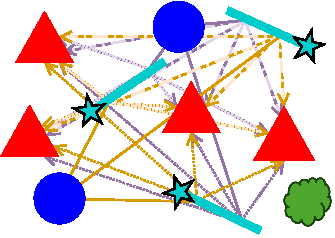
\includegraphics[height=1cm]{img/full_sim.pdf}
    \end{textblock*}
    \footnotesize %
    \begin{columns}
        \begin{column}{0.4\textwidth}
            \begin{block}{\centering \footnotesize \alert{Radar Parameters}}
                \begin{minipage}{0.25\linewidth}
                    \centering \tiny Gain 
                    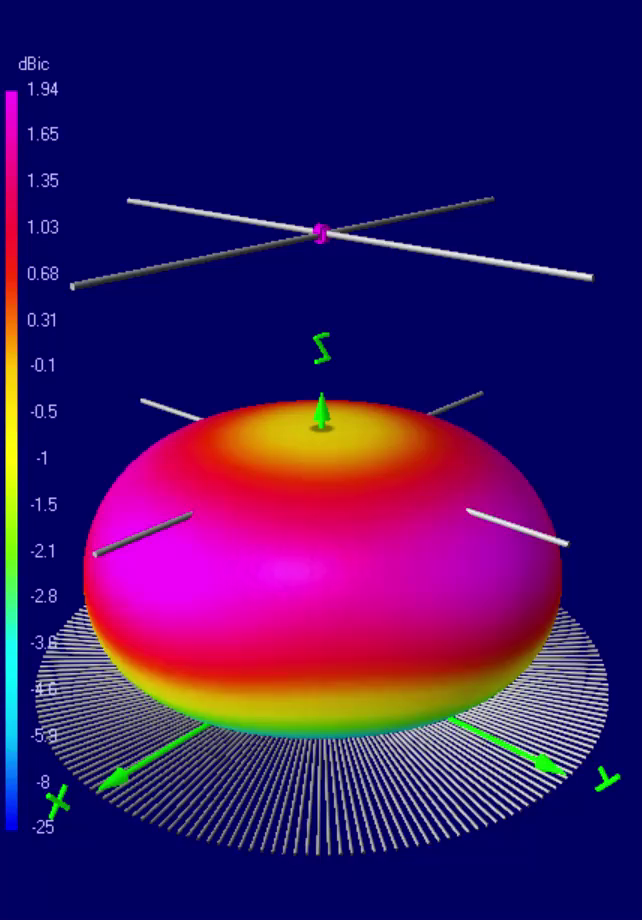
\includegraphics[width=\linewidth]{img/tot_gain/tot_gain.png}
                \end{minipage} %
                \begin{minipage}{0.25\linewidth}
                    \centering \tiny Polarization 
                    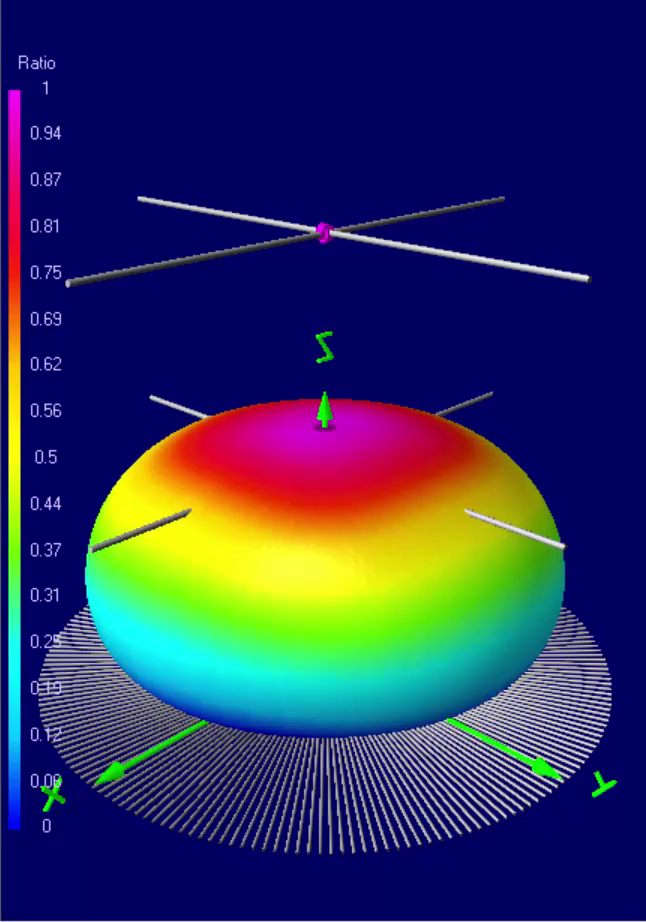
\includegraphics[width=\linewidth]{img/axial_ratio/axial_ratio.png}
                \end{minipage} %
                \begin{minipage}{0.4\linewidth}
                    {\setlength{\leftmargini}{1em}\begin{itemize} \scriptsize
                        \item[\footnotesize $\bullet$] \(\lambda\): wavelength
                        \item[\footnotesize $\bullet$] \(P_T\): \textcolor{blue}{\textbf{TX}} power
                    \end{itemize}}
                \end{minipage}
            \end{block} \vspace{-5pt} %
            \begin{block}{\centering \footnotesize \alert{Geometric Parameters}}
                { \begin{itemize} \scriptsize
                    \item[\footnotesize $\bullet$] \textcolor{blue}{\textbf{TX}}, \textcolor{red}{\textbf{RX}}, meteor head locations
                    \item[\footnotesize $\bullet$] Trail orientation %
                \end{itemize}} \vspace{-5pt}%
            \end{block} \vspace{-5pt} %
            \begin{block}{\centering \footnotesize \alert{Plasma Parameters}}
                {\begin{itemize} \scriptsize
                    \item[\footnotesize $\bullet$] \(q_{max}\): electron line density
                    \item[\footnotesize $\bullet$] \(l_\perp\): trail width
                    \item[\footnotesize $\bullet$] \(l_\parallel\): trail correlation length
                \end{itemize} \vspace{-5pt}}
            \end{block}
        \end{column}
        \begin{column}{0.7\textwidth}
            {\tiny \begin{align*} 
                P_{RX} & = \underset{\substack{\text{Radar Equation,} \\ \text{single electron}}}{\tcbhighmath[colback=blue!10, colframe=blue!70!black, sharp corners, left=0mm, right=0mm]{\frac{P_T G_T G_R \lambda ^2}{(4 \pi)^3 R_T^2 R_R^2} \sigma_{e}}}  \left( \underset{\substack{\text{\# scattering} \\ \text{electrons}}}{ \tcbhighmath[colback=orange!10, colframe=orange!70!black, sharp corners, left=0mm, right=0mm]{N_e}} \right)^2  \ \underset{\substack{\text{Initial trail radius}}}{\tcbhighmath[colback=purple!10, colframe=purple!80, sharp corners, left=0mm, right=0mm]{\e^{-2k^2 \cos^2(\phi) l_{\perp}^2}}}  \\ 
                & = \frac{P_T G_T G_R \lambda ^3r_e^2 \left< \sin^2(\gamma) \right> q_{\max}^2  \e^{-\frac{\delta s^2}{l_{\parallel^2}}}}{16 \pi^2 R_T R_R (R_T + R_R)(1-\sin^2(\phi)\cos^2(\beta))}   \cdot \e^{-\frac{8 \pi^2}{\lambda^2} \cos^2(\phi)(\lambda_\perp)}
            \end{align*}} % 
            \begin{minipage}{0.65\linewidth}
                \centering %
                \adjincludegraphics[width=\linewidth, trim={0 {.2\height} {0.01\width} {.22\height}},clip]{img/GIP_expect.pdf}            
            \end{minipage} %
            \begin{minipage}{0.3\linewidth}
                \begin{tcolorbox}[width = \linewidth, boxrule=0pt,colback=yellow,arc=0pt,auto outer arc,left=0pt,right=0pt,boxsep=2pt]
                    \raggedright \(P_{RX}\) calculated for every meteor using each \textcolor{blue}{\textbf{TX}}-\textcolor{red}{\textbf{RX}} link
                \end{tcolorbox}
            \end{minipage}
            
        \end{column}
    \end{columns}
\end{frame}